% Inside the Mooncake metadata master (standalone figure from slide 2).
% Build: lualatex master_internals.tex
\documentclass{article}
\usepackage{fontspec}
\setsansfont{Helvetica}
\setmonofont{Menlo}[Scale=0.9]
\renewcommand{\familydefault}{\sfdefault}
\usepackage{tikz}
\usetikzlibrary{arrows.meta}
\usepackage{enumitem}
\pagestyle{empty}
\definecolor{rpc}{HTML}{B2182B}
\definecolor{subtext}{gray}{0.35}
\begin{document}
\setbox0=\hbox{%
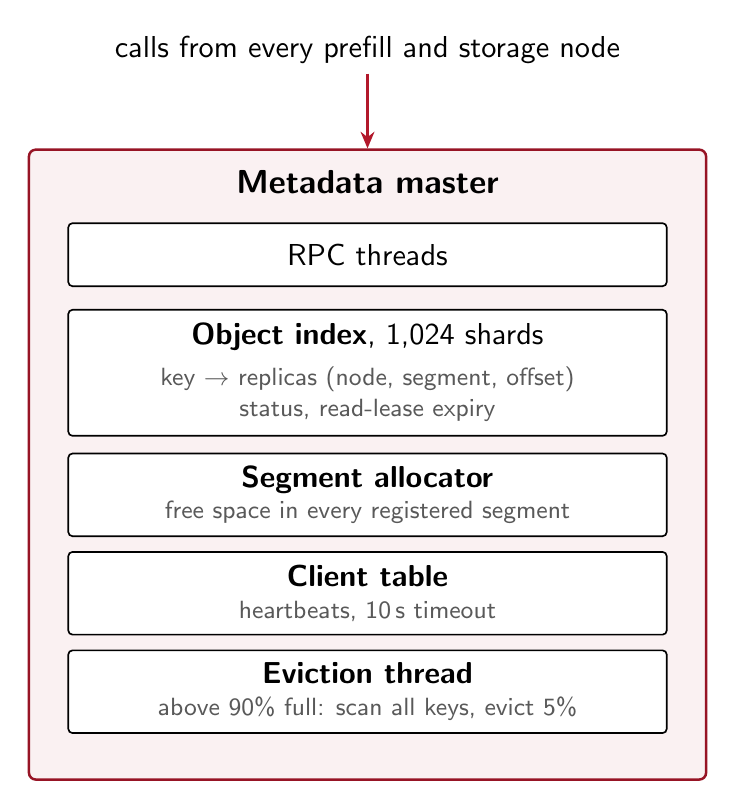
\begin{tikzpicture}[x=1cm,y=1cm]
  % Diagram: inside the master
  \tikzset{part/.style={draw=black, line width=0.6pt, rounded corners=1.5pt, fill=white,
                        align=center, minimum width=7.6cm, font=\fontsize{10.5}{12.5}\selectfont}}
  \node[draw=rpc!85!black, line width=0.9pt, rounded corners=2.5pt, fill=rpc!6,
        minimum width=8.6cm, minimum height=8.0cm, anchor=north] (m) at (19.6,10.9) {};
  \node[anchor=north, font=\fontsize{12}{14}\selectfont\bfseries] at (19.6,10.75) {Metadata master};
  \node[part, minimum height=0.8cm] (rpcth) at (19.6,9.55) {RPC threads};
  \node[part, minimum height=1.6cm] (idx) at (19.6,8.05)
    {\textbf{Object index}, 1,024 shards\\[2pt]
     {\fontsize{9.5}{11.5}\selectfont\color{subtext} key $\rightarrow$ replicas (node, segment, offset)}\\[-1pt]
     {\fontsize{9.5}{11.5}\selectfont\color{subtext} status, read-lease expiry}};
  \node[part, minimum height=1.05cm] (alloc) at (19.6,6.5)
    {\textbf{Segment allocator}\\[-1pt]{\fontsize{9.5}{11.5}\selectfont\color{subtext} free space in every registered segment}};
  \node[part, minimum height=1.05cm] (ctab) at (19.6,5.25)
    {\textbf{Client table}\\[-1pt]{\fontsize{9.5}{11.5}\selectfont\color{subtext} heartbeats, 10\,s timeout}};
  \node[part, minimum height=1.05cm] (evict) at (19.6,4.0)
    {\textbf{Eviction thread}\\[-1pt]{\fontsize{9.5}{11.5}\selectfont\color{subtext} above 90\% full: scan all keys, evict 5\%}};

  % Incoming RPCs from every node
  \draw[-{Stealth[length=6pt,width=5pt]}, line width=1.0pt, draw=rpc] (19.6,11.85) -- (m.north);
  \node[anchor=south, font=\fontsize{10.5}{12.5}\selectfont, align=center] at (19.6,11.85)
    {calls from every prefill and storage node};
\end{tikzpicture}}%
\pdfvariable horigin=0pt
\pdfvariable vorigin=0pt
\pagewidth=\dimexpr\wd0+8pt\relax
\pageheight=\dimexpr\ht0+\dp0+8pt\relax
\shipout\vbox{\kern4pt\hbox{\kern4pt\box0\kern4pt}\kern4pt}
\end{document}
